%%%%%%%%%%%%%%%%%%%%%%%%%%%%%%%%%%%%%%%%%%%%%%%%%%%%%%%%%%%%
%%% LaPreprint: PREPRINT TEMPLATE
%%%%%%%%%%%%%%%%%%%%%%%%%%%%%%%%%%%%%%%%%%%%%%%%%%%%%%%%%%%%

% Here I could talk about what one should do in this document.
% Instead I'll refer you to the explore on your own as check the Github Repo. :-)
% Line spacing is 1.2 by default (can't be smaller).

%%%%%%%%%%%%%%%%%%%%%%%%%%%%%%%%%%%%%%%%%%%%%%%%%%%%%%%%%%%%
%%% PREAMBLE
%%%%%%%%%%%%%%%%%%%%%%%%%%%%%%%%%%%%%%%%%%%%%%%%%%%%%%%%%%%%

% Declare document class
\documentclass[9pt,biorxiv,lineno,blue]{lapreprint}
% Choose between "biorxiv", "medrxiv", "arxiv" and "chemrxiv". Otherwise defaults "Preprint".
% Choose between "blue" and "red" colour scheme. Defaults to "blue".
% Use the "onehalfspacing" option for 1.5 line spacing.
% Use the "doublespacing" option for 2.0 line spacing.
% Use the "lineno" option for line numbers.
% Use the "endfloat" option to place floats after the bibliography.

% Import packages
\usepackage{lipsum}     % Required to insert dummy text
\usepackage[version=4]{mhchem} % For chemical notation
\usepackage{siunitx}    % For SI units
\usepackage{pdflscape}  % For putting pages in landscape mode
\usepackage{rotating}   % For rotating specific elements
\usepackage{textgreek}  % Greek symbols
\usepackage{gensymb}    % Symbols
\usepackage[misc]{ifsym} % For the \Letter symbol
\usepackage{orcidlink}  % For the \orcidlink
\usepackage{listings}   % For inserting code chunks
\usepackage{colortbl}   % For Knitr table colouring
\usepackage{tabularx}   % For making Knitr tables compatible
\usepackage{longtable}  % For multi-page tables
\usepackage{subcaption}
\usepackage{multirow}
\usepackage{snotez}     % For sidenote environments. enotez for endnotes

% Make declarations
\DeclareSIUnit\Molar{M}

% Please note that these options may affect formatting.

%%%%%%%%%%%%%%%%%%%%%%%%%%%%%%%%%%%%%%%%%%%%%%%%%%%%%%%%%%%%
%%% ARTICLE SETUP
%%%%%%%%%%%%%%%%%%%%%%%%%%%%%%%%%%%%%%%%%%%%%%%%%%%%%%%%%%%%

% Paper title
\title{LaPreprint: \\ A Preprint Template for \LaTeX}

% Authors - you can use \orcidlink{} and \authfn{} - see contribution note
\author[ \orcidlink{0000-0002-9998-0058} 1 \Letter]{Mikkel Roald-Arb\o l}
\author[2]{Co-author}

% Affiliations
\affil[1]{School of Life Sciences, University of Sussex}
\affil[2]{University of Somewhere}

% Correspondence
\correspondence{https://github.com/roaldarbol/LaPreprint/issues}{MRA}

% Contribution note
\contribution[\authfn{1}\authfn{2}\authfn{3}]{Here's a few symbols to denote contribution specifics, e.g. authors who contributed equally to the work.}

% Present address of corresponding author
\presentaddress[]{Evolution, Behaviour and Environment, School of Life Sciences, University of Sussex, Biology Road, Brighton, BN1 9RH, United Kingdom}

% Data availability statement, funding and competing interests.
\data[]{Data availability statement. Preprocessed data could be available e.g. on \href{https://zenodo.org/}{Zenodo}.}
\funding[]{MRA was supported by funding from the Leverhulme Foundation. The funders had no role in the template design or decision to publish.}
\compint[]{The author declare no competing interests.}


% Surname of the lead author(s) for the running footer
\leadauthor{Roald-Arb\o l}
\shorttitle{A Preprint Template for \LaTeX}

%%%%%%%%%%%%%%%%%%%%%%%%%%%%%%%%%%%%%%%%%%%%%%%%%%%%%%%%%%%%
%%% ARTICLE START
%%%%%%%%%%%%%%%%%%%%%%%%%%%%%%%%%%%%%%%%%%%%%%%%%%%%%%%%%%%%

\begin{document}
\maketitle
\begin{abstract}
\lipsum[1]
\end{abstract}
\section{Introduction} \label{intro}
Let's begin with some great papers for those interested in radically improving the scientific infrastructure \citep{Pooley2021, Bezuidenhout2021,Brembs2021}.
\lipsum[1-2]
\lipsum[3-4]
\sidenote{This is a sidenote made with the \textbackslash sidenote package. \lipsum[1]}
\section{Methods \& Materials} \label{methods}

\subsection{Behavioural setup}
\lipsum[2]

\subsection{Electrophysiological setup}
\lipsum[2] Figure \ref{fig:setup}.

\begin{figure}
    \centering
    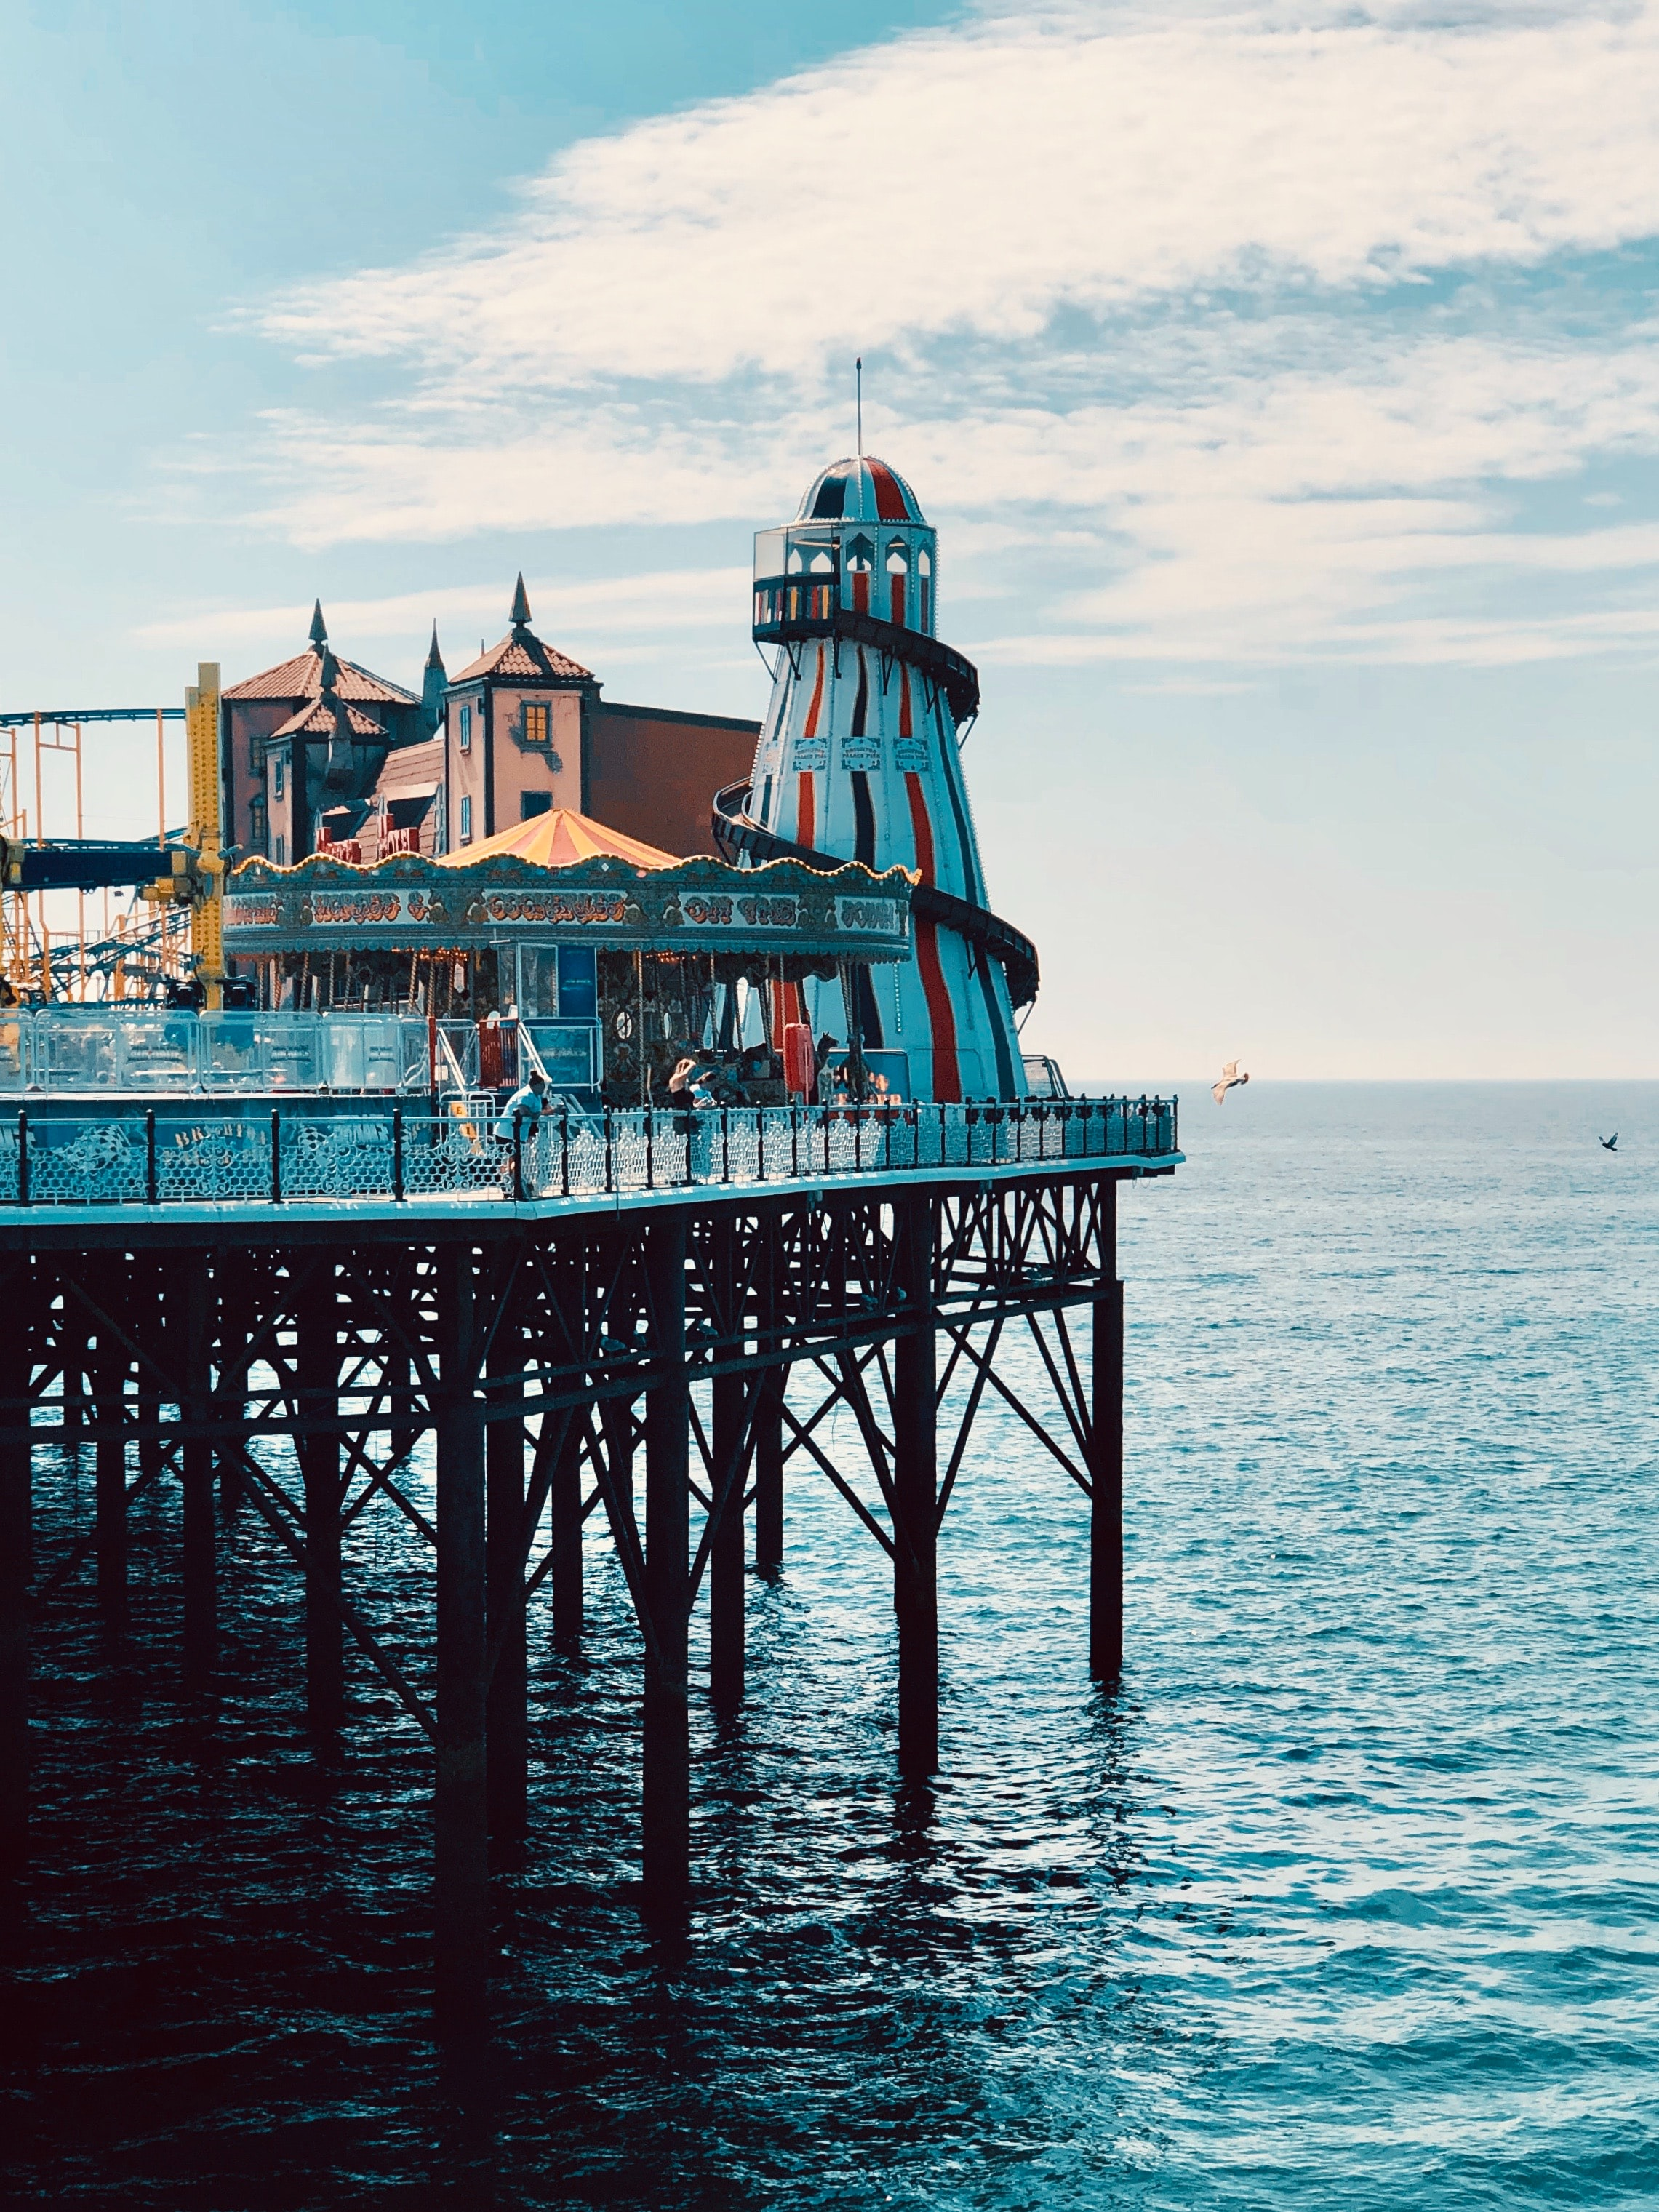
\includegraphics[width=\hsize]{src/figures/brighton.jpeg}
    \caption{
        \textbf{Photo of lovely Brighton by \href{https://unsplash.com/es/@sanekovs?utm_source=unsplash&utm_medium=referral&utm_content=creditCopyText"}{Alex Ovs} on \href{https://unsplash.com/s/photos/brighton?utm_source=unsplash&utm_medium=referral&utm_content=creditCopyText}{Unsplash}.
        }
        \lipsum[1]
    }
    \label{fig:setup}
\end{figure}




\section{Results} \label{results}
\lipsum[1-4]
\section{Discussion} \label{discussion}
\lipsum[1-3]
\subsection{Acknowledgment}
This preprint was created using the LaPreprint template (\url{https://github.com/roaldarbol/lapreprint}) by Mikkel Roald-Arb\o l \textsuperscript{\orcidlink{0000-0002-9998-0058}}.

\subsection{Author contributions}
Consider using a contribution table for clarity. I may add it later.
Conceptualization: E.S., B.H.; Methodology: B.H.; Software: B.H.; Validation: S.R.; Formal analysis: S.R.; Investigation: E.S.; Resources: B.H.; Writing - original draft: E.S.; Writing - review \& editing: S.R., B.H.; Visualization: S.R.; Supervision: B.H.; Project administration: B.H.; Funding acquisition: B.H.
% According to https://journals.biologists.com/jeb/pages/author-contributions

\subsection{Supplementary}
Insert the supplementary text text here.
\bibliography{src/bibliography}

% DON'T EDIT. If "endfloat" option is enabled all floats appear before appendices
\if@endfloat\clearpage\processdelayedfloats\clearpage\fi 


%%%%%%%%%%%%%%%%%%%%%%%%%%%%%%%%%%%%%%%%%%%%%%%%%%%%%%%%%%%%
%%% SUPPLEMENTARY MATERIAL / APPENDICES
%%%%%%%%%%%%%%%%%%%%%%%%%%%%%%%%%%%%%%%%%%%%%%%%%%%%%%%%%%%%

\begin{appendix}
\begin{appendixbox}\label{app:ttt}
    \section{TTT, by Piet Hein}
Problems worthy \\
of attack \\
prove their worth \\
by hitting back. \\
\\
Put up in a place \\
where it's easy to see \\
the cryptic admonishment\\
    T.T.T. \\
\\
When you feel how depressingly \\
slowly you climb, \\
it's well to remember that\\
Things Take Time. \\
\\
The road to wisdom? - Well, it's plain\\
and simple to express: \\
   Err \\
   and err \\
   and err again \\ 
   but less \\
   and less \\
   and less. \\

\end{appendixbox}
\begin{appendixbox}
    \section{Key resources}
Here could be a nice table of your resources. 

% Make your own table style https://tex.stackexchange.com/questions/94799/how-do-i-color-table-columns
\end{appendixbox}
\end{appendix}


%%%%%%%%%%%%%%%%%%%%%%%%%%%%%%%%%%%%%%%%%%%%%%%%%%%%%%%%%%%%
%%% ARTICLE END
%%%%%%%%%%%%%%%%%%%%%%%%%%%%%%%%%%%%%%%%%%%%%%%%%%%%%%%%%%%%

\end{document}
